\chapter{GIVE challenge}
Big part of this master thesis revolves around GIVE challenge. The data I was using to develop the hypothesis where from annotated GIVE experiment. I use GIVE framework to implement and test my hypothesis. Therefore, in this chapter I will describe this academic competition in detail.  

First section will answers basic questions such as what is GIVE challenge, why was it created or what are its interesting properties. In the next section, I will provide a brief history of GIVE challenge together with some of their results. In the third section, the focus will be a detailed description of the shared task and the virtual world of GIVE challenge. Finally, I will describe the dataset I had available for this thesis.

\section{Introduction}
GIVE challenge was a series of Natural Language Generation (NLG) competitions run from November 2008 to March 2012. Participants were developing NLG systems to navigate human subjects in 3D virtual environment through written instructions in real time. The platform for this navigation system was represented as a treasure-hunt game. Multiple evaluation worlds were used in the experiment. More detailed description of the task and the environment is in section \ref{sec:task-give-world}.

\citep{koller2010first} state that one of the goals of GIVE challenge was spawning interest in NLG subfield of computational linguistics, inspired by other competitions in this field such as Recognizing Textual Entailment challenge\footnote{\url{http://pascallin.ecs.soton.ac.uk/Challenges/}} and NIST machine
translation competition\footnote{\url{http://www.itl.nist.gov/iad/mig//tests/mt/}}.

According to \citep{koller2010first}, another important goal was to introduce and explore a new way of evaluating NLG algorithms, techniques and systems in a shared task. More specifically a shared task which was on one hand complex enough to encompass multiple NLG subtasks and, on the other hand, was only concerned with NLG and not any other fields of the computational linguistic.

Three basic approaches to evaluation of NLG systems are comparison with annotated corpora, measuring task performance in experiment and human judges evaluation. \citep{koller2010first} argue the advantages and disadvantages of these evaluation in more depth, therefore I will only provide a brief summary. First approach, where the annotated corpora is also known as a gold-standard, is fast and cheap but the problem lies in language polysemy. The second approach, conducting experiment and measuring task performance on human subjects, is expensive and time consuming. Lastly, using trained human judges is less demanding than the second approach, but for the cost of certainty that the results correspond with the real usage.

GIVE challenge proposes and successfully implements a new approach, in a sense that it wasn't used for NLG before, through Internet-based evaluation. The basic premise is using a client-server software methodology. The client is a program installed on test subject computer, which is easily downloadable from a public website. The client connects through the Internet to a matchmaker server. Matchmaker connects a client to one of the evaluated NLG systems, which itself, can be hosted on a different server. Client and NLG systems then communicate back and forth until the task is finished. Matchmaker finally logs the entire sessions to database. Figure \ref{fig:give-clientserver} shows that architecture in a simple diagram.

\begin{figure}[h]
  \centering
	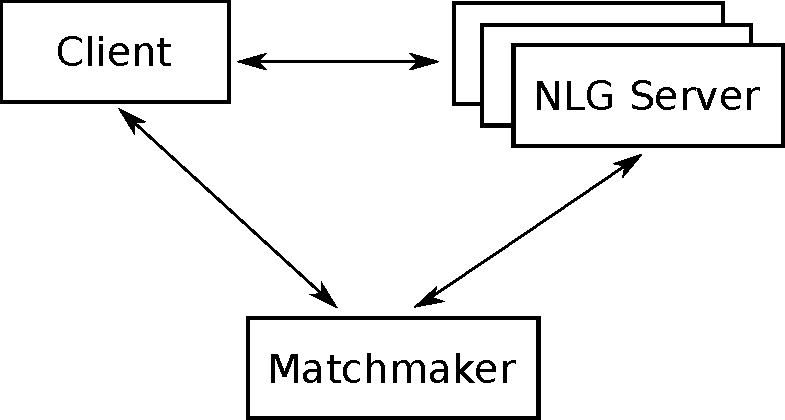
\includegraphics[width=0.7\textwidth]{Images/give-client-servers}
	\caption{Software architecture of GIVE challenge.}
	\label{fig:give-clientserver}
\end{figure}

This approach immediately presents several advantages. It does not require physical presence of the test subject in a laboratory. The subject simply downloads the client from a website and is able to do the experiment at his/her convenience. Second obvious advantage is a scalability. The number of individuals which can parallelly undertake the experiment is only limited by the servers' load. Thanks to the low costs, advertisement becomes the decisive limitation on the number of subjects. Take for example second instalment of GIVE challenge which had up to 1800 participants.

On the other hand, much of the control over the experiment is lost in this approach. For example, the control over subject pool, over failure in task completion or over individuals repeating the experiment, is lost.

In addition to Internet-based evaluation, the GIVE challenge utilizes variety of evaluation measures of both objective and subjective character. Among objective measure are task success rate, number of instructions or time required to finish the task. For subjective measures a questionnaire was used at the end of the session. The questionnaire mostly used a 5 point scale with question as how clear where the instruction or how friendly was the system. Some of the measures intentionally collided with each other, putting emphasize on a certain characteristic of the system. 

 
\section{History of GIVE Challenge}
The first instalment of GIVE challenge (GIVE-1) was publicized in March 2008. \citep{koller2010first} report on this instalment and are the source of following information. For more details please refer to their paper. The data collection period was from November 2008 to February 2009. Four teams participated in this challenge, namely from these universities: University of Texas at Austin, Universidad Complutense de Madrid, University of Twente and Union College. The team from University of Twente submitted two systems, making the final number of systems five.

What is important to note about GIVE-1 is the different world representation from the following instalments. GIVE-1 used discrete square grid for player movement. Player was able to rotate by 90° and work forward and backwards by one square of the grid. That had a major impact on the whole NLG system. Participating teams atleast occasionally used this grid in their references (eg. \textit{move forward three steps}). A movement locked to a discrete grid was after GIVE-1 removed.

Altogether, 1143 valid games were recorded. The demographics featured a majority of males (over 80\%) and wide spread over different countries in the world. Interestingly enough, the system from Austin significantly outperformed all other systems in task completion time. At the same time systems from Union and Madrid outperformed other systems in success rate. That shows the significance of different measures for evaluation. Similar interesting conclusion in both objective and subjective measures can be found in previously mentioned paper. Apart from objective and subjective measures, the report examined influence of English language proficiency and differences between evaluation worlds. The English proficiency had an impact on the task success rate but solely for the least proficient category. The evaluation world also had a significant influence on the task success rate.

Finally, the first instalment also compared the Internet-based evaluation with more standard laboratory evaluation. The conclusion was that Internet-based evaluation provides meaningful results comparable and even more precise in some area to the laboratory setting.

The second instalment (GIVE-2) run from August 2009 (data collection starting in February 2010) to May 2010 and is thoroughly described by \citep{koller2010report}. Following information are based on this paper. Biggest difference to the GIVE-1, which was mentioned previously, is that players were now able to move freely. This made the instruction generation considerably harder. Additionally, the questionnaire was revised and a few new objectives measures were introduced. Evaluation worlds used in GIVE-2 were considerably harder than in GIVE-1. Number of distracting buttons was increased and same-coloured buttons were sometimes next to each other. Also number of alarm tiles was increased. Otherwise, the architecture and the rest of the details stayed the same as in GIVE-1.

This time 1825 games were played over seven NLG systems developed by six teams from: Dublin Institute of Technology,Trinity College Dublin, Universidad Complutense de Madrid,University of Heidelberg, Saarland University and INRIA Grand-Est in Nancy (2 systems).

There was a big drop in success rate, most likely linked to the free movement and the increase of difficulty in the evaluation worlds. Similarly to results in GIVE-1, there was an influence of English proficiency and game world on the task success rate. Additionally, age of the subject played a role in the time required to finish the task and number of actions to finish the task (younger subjects being faster and requiring less actions). The difference between genders in time required to finish the task disappeared in GIVE-2.

Following GIVE-2 was so called Second Second instalment (GIVE-2.5), which kept almost the same settings as GIVE-2. There was just a small addition to objective measures and reduce in a number of subjective questions. The data collection took place between July 2011 and Mar 2012. \citep{striegnitz2011report} reports on the partial results of 536 valid games from July and August 2011, which however constitute a majority of the final number 650 valid games.
\section{Task and GIVE world}
\label{sec:task-give-world}
\section{Dataset}